% The evaluation tree for (2 + 4 * 6) * (3 + 5 + 7), used in Section 1.1.3.
%
% Drawn rather than vendored because upstream's figure_1.1g is the tree for the
% Lisp expression, and Python's differs in exactly one way: arity. Lisp's
% (+ 3 5 7) is ONE application of + to three operands, so upstream's node has
% three operand branches. Python's 3 + 5 + 7 is (3 + 5) + 7 -- two binary
% applications -- so that subtree is one level deeper, with an intermediate 8.
%
% Everything else is deliberately the same as upstream's, including drawing the
% operator as a branch rather than as a label on the node: Python's parse tree
% really does hold the operator as a child (ast.iter_child_nodes on a BinOp
% yields its operator), so the two figures should be directly comparable.
%
% Every value in upstream's figure survives unchanged: 390, 26, 24, 15.

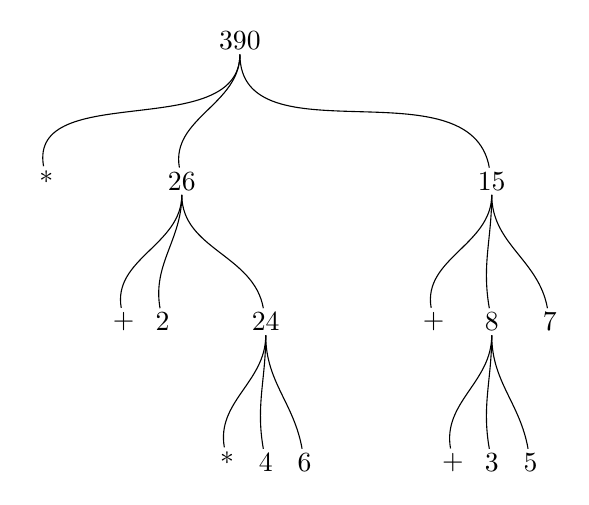
\begin{tikzpicture}[
  x = 0.82cm, y = 1.05cm,
  every node/.style = {inner sep=1.5pt, font=\normalsize},
  branch/.style     = {draw, thin},
]

% level 0
\node (v390) at (-2.4,  0.0) {390};
% level 1
\node (o0)   at (-5.4, -1.7) {*};
\node (v26)  at (-3.3, -1.7) {26};
\node (v15)  at ( 1.5, -1.7) {15};
% level 2
\node (o1)   at (-4.2, -3.4) {+};
\node (n2)   at (-3.6, -3.4) {2};
\node (v24)  at (-2.0, -3.4) {24};
\node (o2)   at ( 0.6, -3.4) {+};
\node (v8)   at ( 1.5, -3.4) {8};
\node (n7)   at ( 2.4, -3.4) {7};
% level 3
\node (o3)   at (-2.6, -5.1) {*};
\node (n4)   at (-2.0, -5.1) {4};
\node (n6)   at (-1.4, -5.1) {6};
\node (o4)   at ( 0.9, -5.1) {+};
\node (n3)   at ( 1.5, -5.1) {3};
\node (n5)   at ( 2.1, -5.1) {5};

\foreach \p/\c in {v390/o0, v390/v26, v390/v15,
                   v26/o1, v26/n2, v26/v24,
                   v15/o2, v15/v8, v15/n7,
                   v24/o3, v24/n4, v24/n6,
                   v8/o4,  v8/n3,  v8/n5}
  \draw[branch] (\p) to[out=-90, in=100] (\c);

\end{tikzpicture}
